\documentclass[11pt]{article}
\usepackage{icmlko}
\begin{document}

\title{짝 둘이 처음으로 갈렸다 --- 규약이 제 일을 했고, 셋째 짝이 급해졌다}
\author{월드모델 실험실}
\date{노트 429 · 2026년 8월 4일}
\maketitle

\begin{abstract}
노트 428이 \textbf{관문은 용량 변경을 아래로 어림한다}는 것을 보이면서
마지막 숙제를 남겼다 --- \emph{$K{=}64$. 노트 396이 ``포화''라 적고 관문으로
물린 용량 손잡이다.} 다시 걸었다.

\begin{center}
\begin{tabular}{lrl}
\hline
 & $K{=}64 - K{=}32$ & \\
\hline
판 (전체 자료, 씨앗 6) & $+0.0005$ & $3/6$ \\
\textbf{비게임 앱 전이} & $\mathbf{+0.0075}$ & $[+0.0053, +0.0094]$ \ $1.000$ \\
\textbf{KR 만화 전이} & $\mathbf{-0.0030}$ & $[-0.0090, +0.0021]$ \ $0.126$ \\
\hline
\end{tabular}
\end{center}

\textbf{판은 사전 등록을 반증했다} --- $+0.002$ 를 요구했는데 $+0.0005$ 다.
노트 396의 ``포화''가 맞고, \textbf{노트 428의 치우침이 $K$ 를 되살리지
못한다}(그 노트가 스스로 적은 한계 그대로 --- 치우침은 변경 둘로 잰 것이지
모든 용량 손잡이에 다 걸리는 법칙이 아니다).

그리고 \textbf{안 본 도메인 둘이 처음으로 반대 부호를 냈다.} 노트 426의
규약이 요구하는 ``둘 이상에서 같은 부호''가 \textbf{미충족}이다 ---
\textbf{안 넣었다.}
\end{abstract}

\section{규약이 제 일을 했다}

이 자리가 규약을 시험한다. 앱 하나만 봤다면 $+0.0075$ 에 $1.000$ 이니
\textbf{넣었을 것이다.} 둘을 요구하는 조항이 그것을 막았다.

두 노트 전에 쓴 조항이고, 그때는 ``짝이 둘뿐이라 조심하자''는 뜻이었지
이런 일이 실제로 날 줄은 몰랐다. \textbf{났다.}

\section{여태 둘은 늘 같은 편이었다}

이번 사이클에 짝 둘을 다 잰 변경이 넷이다.

\begin{center}
\begin{tabular}{lrr}
\hline
변경 & KR 만화 & 비게임 앱 \\
\hline
\texttt{grp} 넣기 & $+0.2950$ & $+0.1053$ \\
깊이 $12-6$ & $+0.0267$ & $+0.0292$ \\
lr $.06 \to .10$ & $+0.0121$ & $+0.0046$ \\
\textbf{$K$ $64-32$} & $\mathbf{-0.0030}$ & $\mathbf{+0.0075}$ \\
\hline
\end{tabular}
\end{center}

셋은 부호도 크기도 맞았다. \textbf{그 일치가 내가 값 매긴 것보다 많은 일을
하고 있었다} --- 셋이 맞았으니 넷째도 맞으리라 여겼고, 그래서 두 짝으로
$0.39$ 짜리 결론까지 지고 왔다(노트 423). 넷째가 갈렸다.

\textbf{셋째 짝이 이제 급하다.} 둘이 갈리면 다수결이 없다. CN 만화는
2025년 이후가 19행이라 못 쓴다 --- 새 도메인을 하나 더 세우거나, 기존
도메인 하나를 학습에서 빼고 전이 시험대로 돌리는 수밖에 없다.

\section{왜 갈렸을까 --- 안 짓는다}

$K$ 는 자루 수다. 늘리면 분산이 준다. 분산이 주는 것이 앱에는 이롭고
만화에는 아닌 까닭을 지어낼 수는 있다 --- 앱은 유보 1{,}600행이고 KR 은
322행이니 어쩌고. \textbf{안 짓는다.} $n{=}2$ 다.

\begin{tabular}{lp{7.0cm}}
\hline
셋째 전이 짝 & 이 노트의 유일한 처방 \\
$K$ & 판에서 포화, 전이에서 갈림 --- \textbf{유지}. 값(적합 시간 두 배)도
안 낼 이유가 된다 \\
노트 428의 치우침 & 용량 손잡이 셋 중 둘(깊이 · lr)에서 보였고 $K$ 에서는
안 보였다. \textbf{법칙이 아니라 경향}으로 적는다 \\
\hline
\end{tabular}

\begin{figure}[h]
\centering
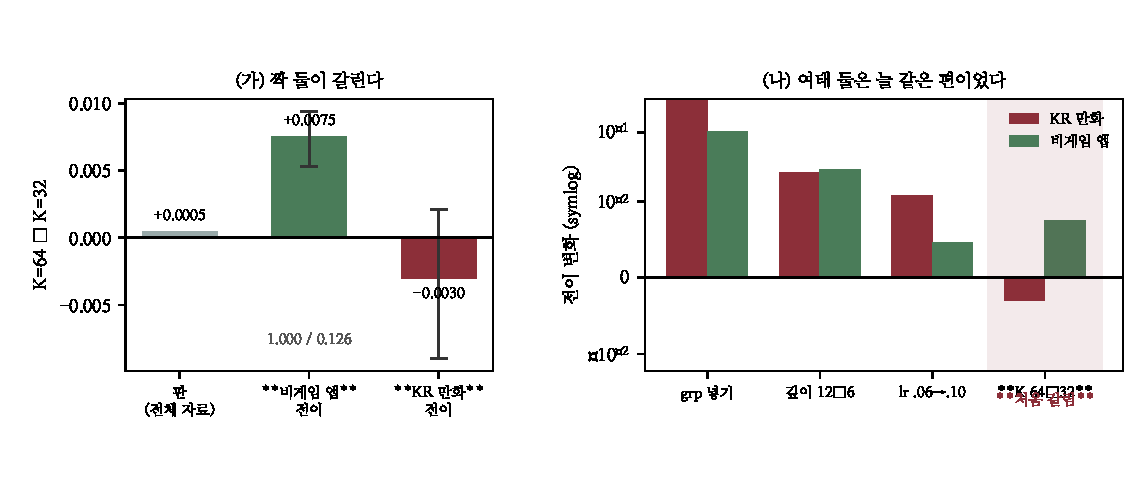
\includegraphics[width=\textwidth]{figs/fig429.pdf}
\caption{(가) 판은 평평하고 짝 둘이 반대로 간다. (나) 이번 사이클의 네
변경 --- 셋은 같은 편, 넷째가 갈린다.}
\end{figure}

\end{document}
